\section{Introduction}
\label{sec:intro}

\begin{figure*}[t]
\centering
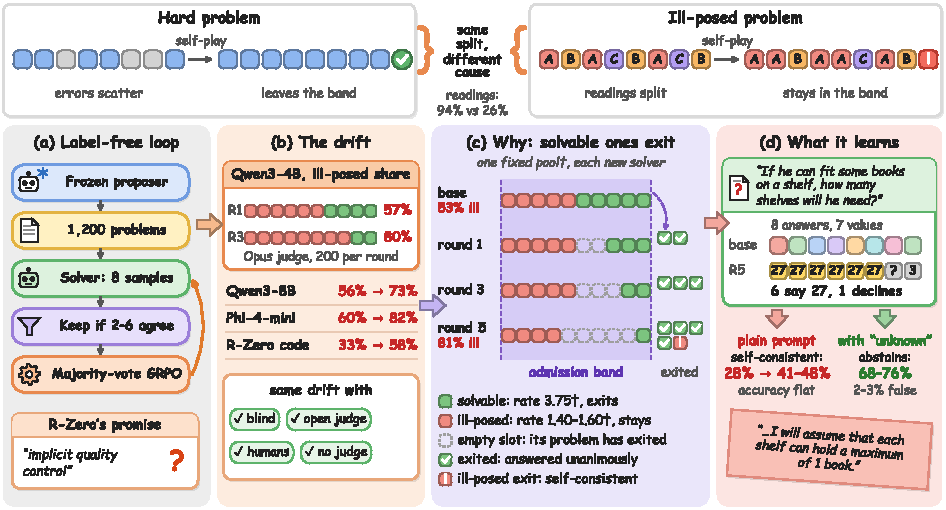
\includegraphics[width=\textwidth,trim=0 0.24bp 0.48bp 0,clip]{figures/overview/overview_paper_svg.pdf}
\caption{Overview. (a)~The label-free loop. (b)~The ill-posed share of admitted problems rises in every model, under every judge (\S\ref{sec:drift}). (c)~On one fixed pool, solvable problems sharpen out of the band; ill-posed ones stay (\S\ref{sec:mechanism}). (d)~The solver answers more unanswerable questions self-consistently and declines more of them in words, and abstains when offered the option (\S\S\ref{sec:accommodation}--\ref{sec:remedies}). Top: errors scatter, readings compete (\S\ref{sec:readings}). $^{\dagger}$Not pre-registered.}
\label{fig:overview}
\end{figure*}

Label-free self-play has become a practical recipe for improving the reasoning of language models \citep{huang2026rzero,zhao2025absolute,fang2025serl,chen2025sqlm}. A proposer writes problems, a solver samples several answers to each, and the solver is trained to agree with its own majority. The recipe needs a rule for which problems to train on, and the common one keeps a problem when the sampled answers disagree: problems always answered the same way teach nothing, and those never agreed on are presumed too hard. R-Zero describes this band of intermediate agreement as \emph{implicit quality control} that filters out ambiguous and ill-posed problems \citep{huang2026rzero}.

The rule conflates two reasons a solver disagrees with itself. A well-posed problem can be hard: computation errors scatter the solver's answers. An ill-posed problem can be read in several ways: a missing quantity must be assumed, two conditions conflict, or a reference is ambiguous, and each reading leads to a different answer. Training on its own majority sharpens the solver: the solvable problems a model writes sharpen toward their answer and leave the band through its upper edge; ill-posed problems start lower and sharpen more slowly, so fewer of them leave. \emph{The band keeps what training has not yet resolved}, and among model-written problems that is mostly the ill-posed ones.

With Qwen3 models of three sizes and Phi-4-mini, the ill-posed share of the admitted curriculum rises in every seed, by 11.5--27 points within two rounds (Figures~\ref{fig:overview}b and~\ref{fig:teaser}a; \S\ref{sec:drift}), also under blind re-judging, an open-weight judge and expert human annotation. In our loop, whose proposer is frozen, the drift is a property of the filter: when successive solvers score one fixed pool, solvable problems leave the band faster than ill-posed ones, and an odds decomposition ties this differential exit exactly to the drift (\S\ref{sec:mechanism}). In the official R-Zero code the curriculum drifts as much, mostly because the challenger, rewarded with the same uncertainty signal, writes more ill-posed questions.

Self-play also changes what the solver does with unanswerable questions (\S\ref{sec:accommodation}). Asked ``If he can fit some books on a shelf, how many shelves will he need?'', the base model gives eight answers spread over seven values; after five rounds, the solver answers 27 in six of eight, because it ``will assume that each shelf can hold a maximum of 1 book'': it accommodates the question's presupposition that an answer exists by inventing the missing premise \citep{lewis1979scorekeeping}. For Qwen3-4B, benchmark accuracy plateaus after the first round while self-consistent answers to unanswerable questions rise from 28\% to 41--48\% by round three, and declines in words from 3\% to 13--22\% of samples (Figure~\ref{fig:overview}d). Most of this rise is majority-vote sharpening, which any label-free curriculum shares; what the drift adds is not established. No label-free admission rule we tested stops the drift, and rewarding ``unknown'' backfires, but offering abstention at test time works (\S\ref{sec:remedies}). We pre-registered 136 predictions (Appendix~\ref{app:prereg}), mark the rest, and release the labelled curricula, judge prompt and probes.
